
%%%%%%%%%%%%%%%%%%%%%%%%%%%%%%%%%%%%%%%%%%%%%%%%%%%%%%%%%%%%%%%%%%%%%
\royslide{Phase Separation - Spinodal Decomposition}{

\royitemizebegin{Initial Evolution}
\item Initial homogeneous blend quenched below critical T
\item Random perturbations anti-diffuse into two phases divided by 
narrow interfaces
\item Gradual coalescence of single-phase regions
\item Additional physics leads to pattern self-assembly
\royitemizeend

\begin{center}
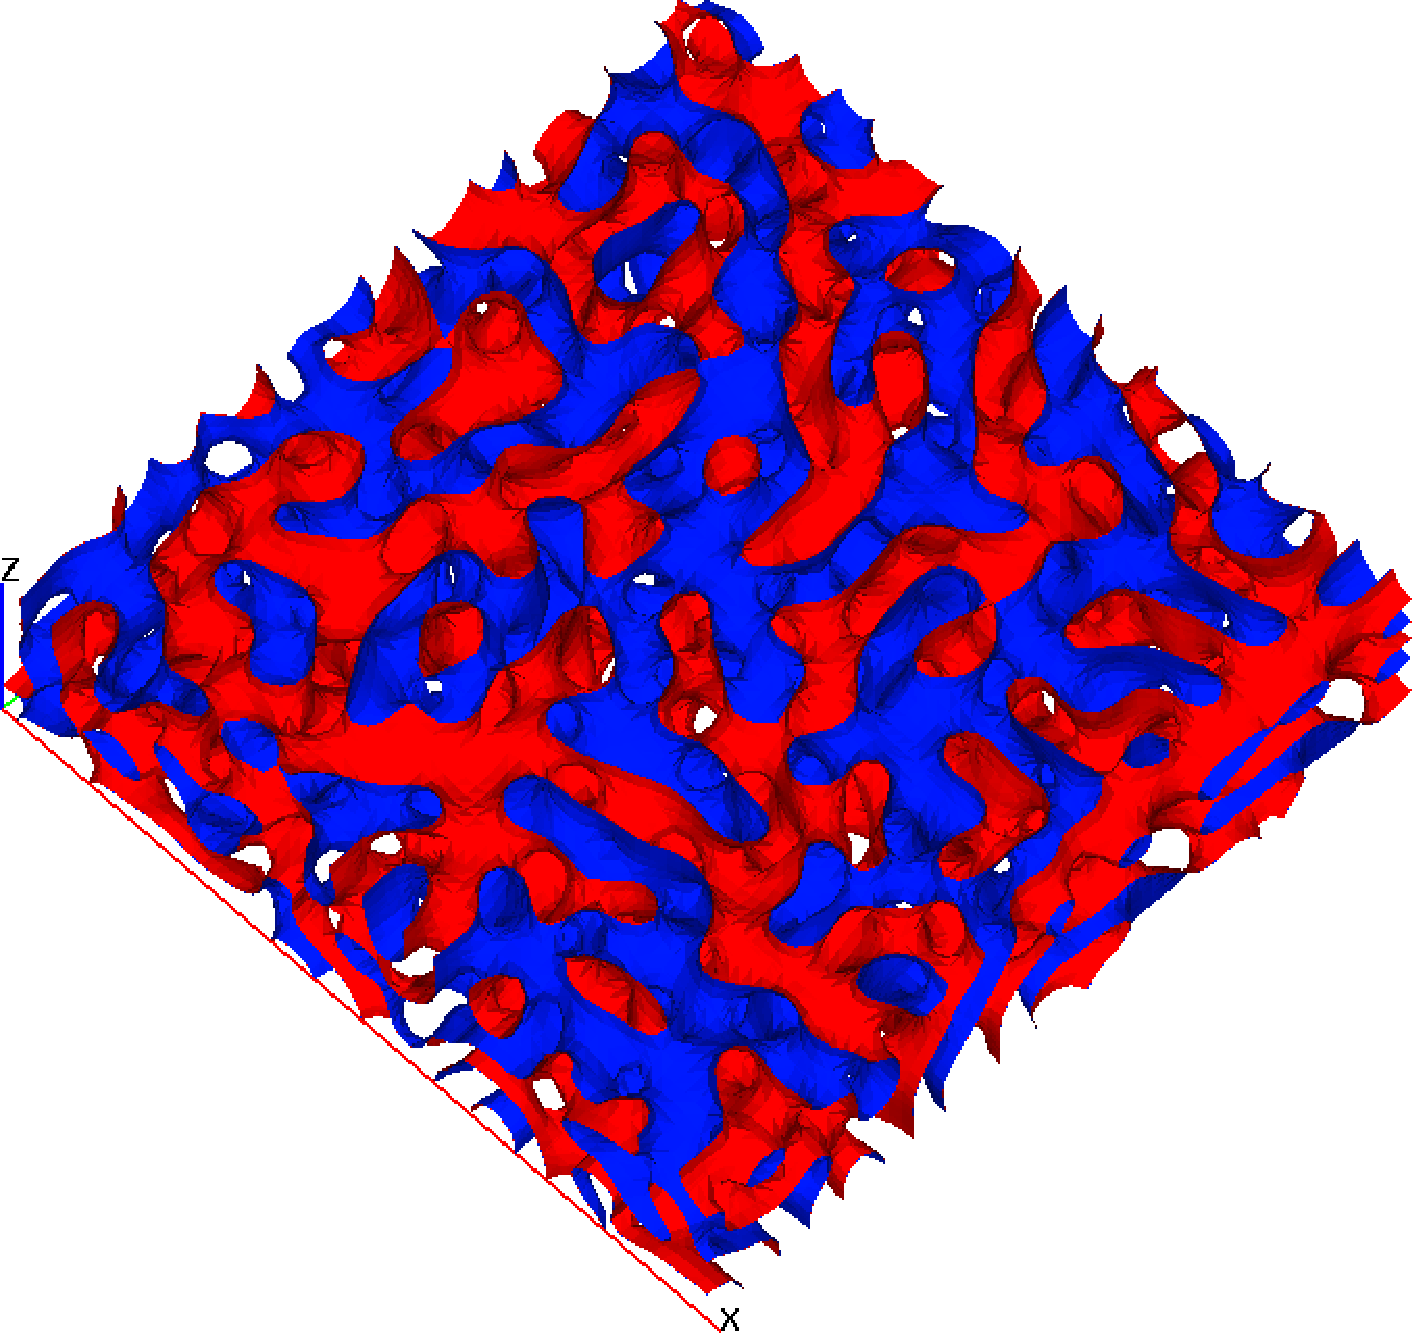
\includegraphics[width=.3\textwidth]{figs/ch3D02-006}
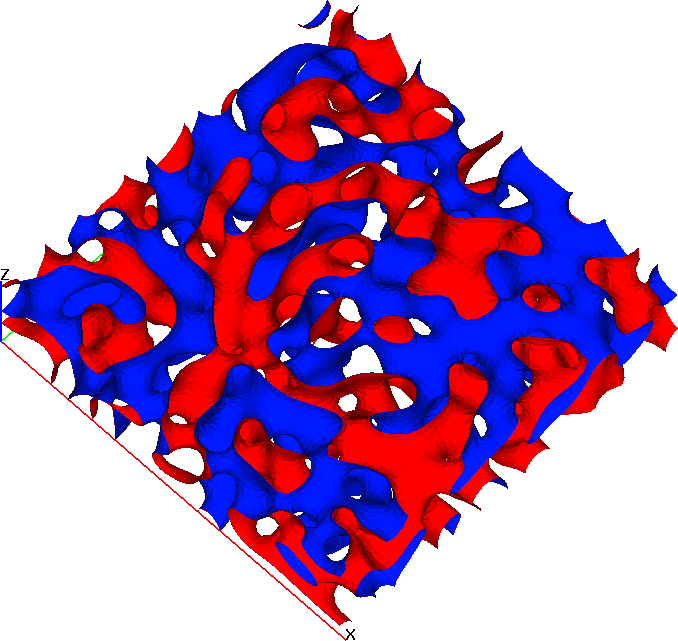
\includegraphics[width=.3\textwidth]{figs/ch3D02-024}
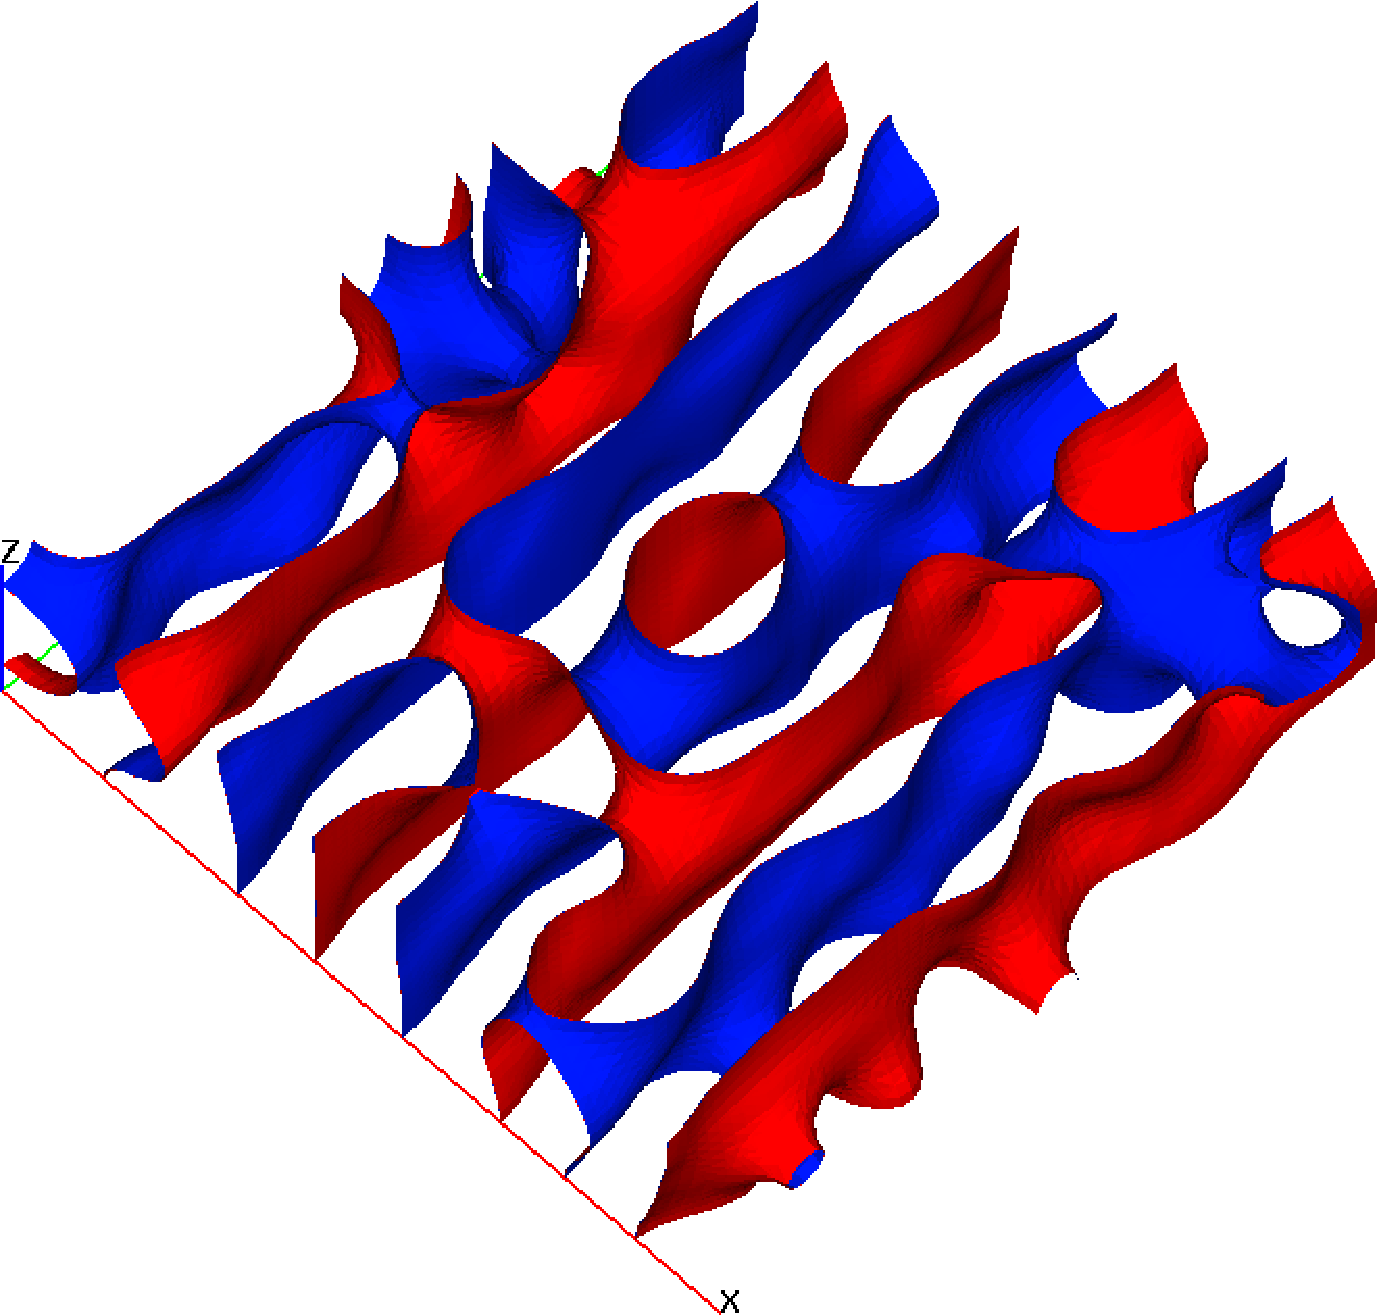
\includegraphics[width=.3\textwidth]{figs/ch3D02-096}
\end{center}
}
